 \باب{بوولین الجبرا}
بوولین الجبرا انگلستان کے   ریاضی  دان جارج بوولی کے نام سے جانا جاتا  ہے، جنہوں نے اس الجبرا کو دریافت کیا۔بوولین الجبرا ذہنی سوچ یعنی منطق کو الجبرائی روپ  میں لکھنے کی صلاحیت رکھتی ہے۔اس لئے  حیرانی کی بات نہیں کہ  کمپیوٹر اسی کو استعمال کرتا ہے۔

\حصہ{بوولین الجبرا کے بنیادی تصورات} \شناخت{حصہ_بوولین_الجبرا_بنیادی_تصورات}
عام الجبرا میں متغیرات استعمال کرتے  ہوئے  تصور کیا جاتا ہے کہ ان کی  قیمت کچھ بھی  ہو سکتی ہے۔مثلاً،  تفاعل   \عددی{z=f(x,y)}،  جہاں   \عددی{x} اور  \عددی{y}  آزاد متغیرات   جبکہ \عددی{z}  تابع متغیر ہے،  میں متغیرات کی چند   ممکنہ قیمتیں درج ذیل     ہیں۔
\begin{center}
\begin{otherlanguage}{english}
\begin{tabular}{CC|C}
x&y&z\\
\toprule
0&0&0\\
1&2&5\\
2&1&4\\
3&2&7\\
2&2&6\\
3&1&5
\end{tabular}
\end{otherlanguage}
\end{center}
اس تفاعل جس  کو ایک نا مکمل جدول کے روپ میں  پیش کیا گیا ہے  کا الجبرائی روپ   درج ذیل ہے۔
 \begin{align*}
 z=x+2y
 \end{align*}
اس کے برعکس،  بوولین الجبرا میں متغیرات کی صرف دو ممکنہ قیمتیں ہیں۔ ان دو قیمتوں کو عموماً   \عددی{0} (صفر)    اور   \عددی{1} (ایک)   سے ظاہر کیا جاتا ہے۔بوولین تفاعل کی چند مثالوں پر غور کرتے ہیں۔

\جزوحصہ{منطقی ضرب}
تصور کریں  \عددی{X}  اور \عددی{Y}  آزاد بوولین متغیرات ہیں،  جبکہ \عددی{Z}  ان کا تابع بوولین متغیر \عددی{Z=f(X,Y)} ہے۔ چونکہ \عددی{X}  بوولین متغیر ہے،  لہٰذا اس کی ممکنہ قیمتیں صرف \عددی{0} اور \عددی{1} ہیں۔اسی طرح \عددی{Y}  بھی بوولین متغیر ہے،  لہٰذا اس کی قیمت  بھی صرف  \عددی{0} اور \عددی{1} ہو سکتی ہے۔تابع متغیر \عددی{Z}بھی بوولین متغیر ہے۔اس طرح اگرچہ اس کی قیمت \عددی{X} اور \عددی{Y} کی تابع ہے،   اس کے باوجود \عددی{Z} کی قیمت  صرف  \عددی{0} یا \عددی{1}    ہی ہو سکتا ہے۔ متغیرات \عددی{X} اور \عددی{Y}  درج ذیل چار ممکنہ ترتیب میں پائے جا سکتے ہیں۔
\begin{center}
\begin{otherlanguage}{english}
\begin{tabular}{CC}
X&Y\\
\toprule
0&0\\
0&1\\
1&0\\
1&1
\end{tabular}
\end{otherlanguage}
\end{center}
ان چار ممکنہ صورتوں میں \عددی{Z} کی   قیمت \عددی{0} یا \عددی{1}  ہوگی۔

آئیں، جدول \حوالہ{جدول_بوولین_جمع} میں پیش کیے گئے منطقی تفاعل پر غور کرتے ہیں جس کی تمام ممکنہ قیمتیں اس جدول میں دی گئی ہیں۔
\begin{table}
\centering
\begin{otherlanguage}{english}
\begin{tabular}{CC|C}
X&Y&Z\\
\toprule
0&0&0\\
0&1&0\\
1&0&0\\
1&1&1
\end{tabular}
\end{otherlanguage}
\caption{دو   متغیر منطقی ضرب}
\label{جدول_بوولین_جمع}
\end{table}
اس مثال میں تابع متغیر \عددی{Z}   کی قیمت صرف   اس وقت   \عددی{1}  ہے جب \عددی{X}   اور \عددی{Y}  دونوں کی قیمت \عددی{1}   ہے۔یہی قیمتیں \عددی{X}  اور \عددی{Y}  کی سادہ ضرب \عددی{X\cdot Y}  سے بھی حاصل ہوتی ہیں (ذیل دیکھیں)۔
\begin{align*}
0\cdot 0&=0\\
0\cdot 1&=0\\
1\cdot 0&=0\\
1\cdot 1&=1
\end{align*}
اسی کی بنا پر جدول \حوالہ{جدول_بوولین_جمع} میں پیش     تفاعل (اور  عمل)  کو  بوولین ضرب یا منطقی ضرب   کہتے ہیں۔ بوولین ضرب کو آزاد متغیرات کے درمیان نقطہ    \قول{\عددی{\cdot}} سے یا    آزاد متغیرات کو قریب قریب  لکھنے سے ظاہر کیا جاتا ہے۔یوں بوولین ضرب   درج ذیل لکھا  جائے گا۔
\begin{gather}
\begin{aligned}
Z&=X\cdot Y\\
Z&=XY&\text{\RL{\small{(بوولین ضرب)}}}
\end{aligned}
\end{gather}
منطقی ضرب  کے  تصور کو وسعت دے کر    متعدد آزاد متغیرات کے لئے بیان کیا جا سکتا ہے۔ منطقی ضرب کی عمومی تعریف پیش کرتے ہیں۔

\ابتدا{تعریف}
منطقی ضرب  اس صورت \عددی{1} دیگا جب تمام آزاد متغیرات کی قیمت \عددی{1} ہو۔
\انتہا{تعریف}

 جدول  \حوالہ{شکل_بوولین_ضرب_دو_متغیر_گیٹ} کو مثال بناتے ہیں۔ اس طرح کے جدول میں آزاد متغیرات کی تمام ممکنات لکھنے (یعنی آزاد متغیرات کے خانے پر کرنے)  کی خاطر  مداخل \عددی{XY}  کو    ثنائی عدد کے ہندسے تصور کر کے، جدول کے مطلوبہ خانوں میں    صفر \عددی{(00)}  تا  تین  \عددی{(11)} گنتی لکھیں۔یوں پہلے صف میں \عددی{XY} کی جگہ \عددی{00}، دوسری صف میں \عددی{01}، تیسرے میں \عددی{10} اور آخری میں \عددی{11} لکھا جائے گا۔
 
تین آزاد متغیرات کے منطقی ضرب تفاعل \عددی{Z=ABC}  کو جدول \حوالہ{جدول_بوولین_تین_متغیر_بوولین_ضرب} میں پیش کیا گیا ہے۔آپ دیکھ سکتے ہیں کہ جدول کے تین  مداخل  کے خانوں میں صفر \عددی{(000)} تا سات \عددی{(111)} گنتی لکھی گئی ہے (جو تین ہندسوں  کے ثنائی اعداد ہیں  )۔
\begin{table}
\centering
\begin{otherlanguage}{english}
\begin{tabular}{CCC|C}
A&B&C&Z\\
\toprule
0&0&0&0\\
0&0&1&0\\
0&1&0&0\\
0&1&1&0\\
1&0&0&0\\
1&0&1&0\\
1&1&0&0\\
1&1&1&1
\end{tabular}
\end{otherlanguage}
\caption{تین متغیر بوولین ضرب}
\label{جدول_بوولین_تین_متغیر_بوولین_ضرب}
\end{table}

\جزوحصہ{منطقی جمع}
دو آزاد متغیرات کے بوولین تفاعل کی ایک اور مثال لیتے ہیں جس کو جدول \حوالہ{جدول_بوولین_جمع_منطقی}  میں پیش کیا گیا ہے۔
\begin{table}
\centering
\begin{minipage}[t]{0.45\textwidth}
\centering
\begin{otherlanguage}{english}
\begin{tabular}{CC|C}
X&Y&Z\\
\toprule
0&0&0\\
0&1&1\\
1&0&1\\
1&1&1
\end{tabular}
\end{otherlanguage}
\caption{دو متغیر منطقی جمع}
\label{جدول_بوولین_جمع_منطقی}
\end{minipage}\hfill
\begin{minipage}[t]{0.45\textwidth}
\centering
\begin{otherlanguage}{english}
\begin{tabular}{CC|C}
X&Y&S\\
\toprule
0&0&0\\
0&1&1\\
1&0&1\\
1&1&2
\end{tabular}
\end{otherlanguage}
\caption{دو ثنائی اعداد کا سادہ مجموعہ}
\label{جدول_بوولین_جمع_سادہ}
\end{minipage}
\end{table}
اب \عددی{Z}   اس صورت   \عددی{1} کے برابر ہے جب \عددی{X}  یا \عددی{Y} یا دونوں کی قیمت  \عددی{1}   ہو۔اس بوولین عمل کو  بوولین جمع یا منطقی جمع  کہتے ہیں۔

آزاد متغیرات  \عددی{X}  اور \عددی{Y} کا  (روز مرہ) سادہ    الجبرائی مجموعہ  \عددی{S=X+Y} جدول \حوالہ{جدول_بوولین_جمع_سادہ} میں پیش کیا گیا ہے۔

جدول   \حوالہ{جدول_بوولین_جمع_منطقی}  اور جدول  \حوالہ{جدول_بوولین_جمع_سادہ}  کے اولین تین نتائج ایک جیسے ہیں۔اس مشابہت کی  بنا   جدول \حوالہ{جدول_بوولین_جمع_منطقی}  میں دیے  گئے بوولین تفاعل کو بوولین جمع  یا منطقی جمع  کہتے ہیں اور اس بوولین تفاعل کو جمع کے نشان \قول{\عددی{+}} سے ہی ظاہر کیا جاتا ہے۔یوں جدول   \حوالہ{جدول_بوولین_جمع_منطقی}میں پیش بوولین جمع  تفاعل درج ذیل لکھا جائے گا۔
\begin{align}
Z&=X+Y&\text{\RL{\small{(بوولین جمع)}}}
\end{align}
یہ  بوولین تفاعل کی مساوات ہے جس کو عام الجبرائی جمع ہرگز نہ سمجھا جائے۔بالخصوص،   بوولین جمع کرتے وقت یاد رہے کہ \عددی{1+1=1}ہے۔

بوولین جمع کے  تصور کو وسعت دے کر   متعدد  آزاد متغیرات کے لئے  بیان کیا جا سکتا ہے۔ بوولین جمع کی عمومی تعریف درج ذیل ہے۔

\ابتدا{تعریف}
منطقی جمع   اس صورت \عددی{1} دیگا  جب  آزاد متغیرات میں کم  سے کم ایک متغیر کی قیمت \عددی{1} ہو۔
\انتہا{تعریف}

تین متغیر منطقی جمع تفاعل \عددی{Z=A+B+C}   جدول  \حوالہ{جدول_بوولین_تین_متغیر_جمع} میں پیش کیا گیا ہے۔
\begin{table}
\centering
\begin{minipage}[b]{0.45\textwidth}
\centering
\begin{otherlanguage}{english}
\begin{tabular}{CCC|C}
A&B&C&Z\\
\toprule
0&0&0&0\\
0&0&1&1\\
0&1&0&1\\
0&1&1&1\\
1&0&0&1\\
1&0&1&1\\
1&1&0&1\\
1&1&1&1
\end{tabular}
\end{otherlanguage}
\caption{تین متغیر منطقی جمع}
\label{جدول_بوولین_تین_متغیر_جمع}
\end{minipage}\hfill
\begin{minipage}[b]{0.45\textwidth}
\centering
\begin{otherlanguage}{english}
\begin{tabular}{C|C}
X&Z\\
\toprule
0&1\\
1&0
\end{tabular}
\end{otherlanguage}
\caption{منطقی نفی یا متمم}
\label{جدول_بوولین_نفی}
\end{minipage}
\end{table}
یاد رہے کہ  تین آزاد متغیرات کے منطقی جمع  کا الجبرائی جمع کے ساتھ کوئی تعلق نہیں۔یہاں جمع کی علامت  بوولین جمع کو ظاہر کرتی ہے لہٰذا یہاں    \عددی{1+1+1=1} ہو گا۔


\جزوحصہ{منطقی نفی}
بوولین تفاعل \عددی{ Z=f(X)} کی  تیسری مثال  لیتے ہیں جہاں  آزاد متغیر \عددی{X}  اور تابع متغیر \عددی{Z} کا تعلق جدول \حوالہ{جدول_بوولین_نفی} میں پیش کیا گیا ہے۔

  اس تفاعل کو بوولین نفی  کہتے ہیں۔آپ دیکھ سکتے ہیں کہ درحقیقت، تابع متغیر \عددی{Z}،  آزاد متغیر کا متمم ہے۔یوں بوولین نفی درج ذیل لکھا جا سکتا ہے۔

\begin{align}
Z&=\overline{X}&\text{\RL{\small{(بوولین نفی یا متمم)}}}
\end{align}
بوولین نفی     صرف   ایک آزاد متغیر کے لئے  بیان کیا جا سکتا ہے، اور اس کی تعریف درج ذیل ہے۔

\ابتدا{تعریف}
بوولین نفی آزاد متغیر کا متمم دیتا ہے۔
\انتہا{تعریف}

\جزوحصہ{منطقی بلا شرکت جمع}
دو آزاد متغیرات کا ایسا  بوولین تفاعل جدول \حوالہ{جدول_بوولین_دو_بلا_شرکت}  میں دکھایا گیا ہے، جس کا   تابع متغیر اس صورت  \عددی{1} ہے جب صرف ایک  آزاد متغیر \عددی{1} ہو۔ یہ  دو متغیر بوولین بلا شرکت جمع ہے۔
\begin{table}
\centering
\begin{minipage}[b]{0.45\textwidth}
\centering
\begin{otherlanguage}{english}
\begin{tabular}{CC|C}
A&B&Z\\
\toprule
0&0&0\\
0&1&1\\
1&0&1\\
1&1&0
\end{tabular}
\end{otherlanguage}
\caption{دو متغیر منطقی  بلا شرکت جمع}
\label{جدول_بوولین_دو_بلا_شرکت}
\end{minipage}\hfill
\begin{minipage}[b]{0.45\textwidth}
\centering
\begin{otherlanguage}{english}
\begin{tabular}{CCC|C}
A&B&C&Z\\
\toprule
0&0&0&0\\
0&0&1&1\\
0&1&0&1\\
0&1&1&0\\
1&0&0&1\\
1&0&1&0\\
1&1&0&0\\
1&1&1&1
\end{tabular}
\end{otherlanguage}
\caption{تین متغیر بوولین بلا شرکت جمع}
\label{جدول_بوولین_تین_متغیر_بلا_شرکت}
\end{minipage}
\end{table}
اس تصور کو  متعدد آزاد متغیرات تک وسعت دے کر بیان کرتے ہیں۔

\ابتدا{تعریف}
طاق تعداد کے آزاد متغیرات \عددی{1} ہو نے کی صورت میں بوولین بلا شرکت   کا تابع متغیر \عددی{1} ہو گا۔
\انتہا{تعریف}

تین آزاد متغیر  بلا شرکت جمع تفاعل کو جدول  \حوالہ{جدول_بوولین_تین_متغیر_بلا_شرکت} میں پیش کیا گیا ہے۔



دو اور تین آزاد متغیر بوولین بلا شرکت  کی مساوات درج ذیل ہوں گی۔
\begin{gather}
\begin{aligned}
Z&=A\oplus B&\text{\RL{\small{(دو آزاد متغیر بلا شرکت جمع)}}}\\
Z&=A\oplus B\oplus C&\text{\RL{\small{(تین آزاد متغیر بلا شرکت جمع)}}}
\end{aligned}
\end{gather}

\جزوحصہ{منطقی ضد  بلا شرکت  جمع}
 بوولین بلا شرکت جمع تفاعل کا نفی  (یعنی متمم)  لینے سے بوولین  ضد   بلا شرکت  جمع    حاصل ہو گا،  جو دو اور تین آزاد متغیرات کے لئے درج ذیل لکھا جاتا ہے۔
\begin{gather}
\begin{aligned}
Z&=\overline{A\oplus B}\\
Z&=\overline{A\oplus B\oplus C}&\text{\RL{\small{(تین متغیر منطقی ضد بلا شرکت جمع)}}}
\end{aligned}
\end{gather}
 جدول \حوالہ{جدول_بوولین_دو_بلا_شرکت} اور جدول \حوالہ{جدول_بوولین_تین_متغیر_بلا_شرکت} میں تابع متغیر نفی کرنے سے   بالترتیب دو اور تین  بوولین  ضد بلا شرکت  تفاعل حاصل ہوں گے جنہیں جدول \حوالہ{جدول_بوولین_دو_متمم_بلا_شرکت} اور جدول \حوالہ{جدول_بوولین_تین_متغیرمتمم_بلا_شرکت} میں پیش کیا گیا ہے۔
\begin{table}
\centering
\begin{minipage}[b]{0.45\textwidth}
\centering
\begin{otherlanguage}{english}
\begin{tabular}{CC|C}
A&B&Z\\
\toprule
0&0&0\\
0&1&1\\
1&0&1\\
1&1&0
\end{tabular}
\end{otherlanguage}
\caption{دو متغیر منطقی ضد   بلا شرکت جمع}
\label{جدول_بوولین_دو_متمم_بلا_شرکت}
\end{minipage}\hfill
\begin{minipage}[b]{0.45\textwidth}
\centering
\begin{otherlanguage}{english}
\begin{tabular}{CCC|C}
A&B&C&Z\\
\toprule
0&0&0&0\\
0&0&1&1\\
0&1&0&1\\
0&1&1&0\\
1&0&0&1\\
1&0&1&0\\
1&1&0&0\\
1&1&1&1
\end{tabular}
\end{otherlanguage}
\caption{تین متغیر بوولین ضد  بلا شرکت جمع}
\label{جدول_بوولین_تین_متغیرمتمم_بلا_شرکت}
\end{minipage}
\end{table}
\حصہ{برقی تاروں میں جوڑ کی وضاحت}
  درج ذیل  شکل  پر غور کریں جس  میں دو برقی تاروں کے بیچ  جوڑ کی وضاحت کی گئی ہے۔
  
  جہاں ایک تار دوسری تار کے   اوپر سے گزرتی ہو  اور  دونوں آپس میں  جڑی ہوں،   وہاں  جوڑ کے مقام پر نقطے  کا نشان لگایا جاتا ہے۔ایسی صورت میں انہیں ایک  تار تصور کیا جائے۔
  
   جہاں تاریں  آپس میں جڑی نہ ہوں وہاں انہیں بغیر نقطے کے نشان سے   ایک دوسری کے اوپر سے گزرتا دکھایا جاتا ہے۔ نقطہ کے نشان کی غیر موجودگی میں ان تاروں کو دو علیحدہ اور بلا جوڑ  تاریں سمجھا جائے۔

 تیسری صورت بھی شکل میں دکھائی گئی ہے جہاں غلط فہمی کا  امکان نہیں پایا جاتا۔اس میں ایک تار کا سر دوسری تار پر ختم ہو تا ہے۔ ایسی صورت میں انہیں ایک  تار تصور کیا جائے  (یعنی یہ دونوں آپس میں جڑی ہیں) ۔
\begin{center}
\begin{tikzpicture}
\draw(-1,0)--(1.5,0);
\draw(0,0)--++(0,-0.75)--++(1,0);
\draw(0,-1)node[above left]{\text{\RL{جوڑ}}};
\end{tikzpicture}\quad\quad
\begin{tikzpicture}
\draw(-1,0)--(1.5,0);
\draw(0,1)--(0,-1);
\draw(0,-1)node[above right]{\text{\RL{بلا جوڑ}}};
\end{tikzpicture}\quad \quad 
\begin{tikzpicture}
\draw(-1,0)--(1.5,0);
\draw(0,1)--(0,0)node[circ]{}--(0,-1);
\draw(0,-1)node[above right]{\text{\RL{جوڑ}}};
\end{tikzpicture}
\end{center}

\حصہ{عددی گیٹ}
 بوولین الجبرا کے تین اہم ترین تفاعل پر حصہ \حوالہ{حصہ_بوولین_الجبرا_بنیادی_تصورات} میں  غور  کیا گیا۔یہ  تفاعلات  عددی  برقیات  میں کلیدی کردار ادا کرتے ہیں، جہاں انہیں  عددی ادوار کی مدد سے جامہ   پہنایا  جاتا ہے۔یہ مخصوص عددی ادوار،  عددی گیٹ  کہلاتے ہیں۔
 
\جزوحصہ{ضرب گیٹ}
منطقی (بوولین)  ضرب   تفاعل کو   ضرب گیٹ سے حاصل کیا جاتا ہے،  جو شکل  \حوالہ{شکل_بوولین_ضرب_گیٹ}  میں دکھایا گیا ہے۔ آزاد متغیرات،  \عددی{X}  اور \عددی{Y}،   ضرب گیٹ کی  بائیں جانب ہیں  جبکہ تابع متغیر، \عددی{Z}،  دائیں جانب  ہے۔  آزاد متغیرات کو مداخل  جبکہ تابع متغیر  کو مخارج کہتے ہیں۔دو متغیر  ضرب گیٹ (دو مداخل ضرب  گیٹ)  کے دو مداخل اور ایک مخارج ہو   گا۔
	
\begin{figure}
\centering
\begin{minipage}[b]{0.40\textwidth}
\centering
\begin{tikzpicture}
\draw(0,0)node[and port](and1){};
\draw(and1.in 1)node[left]{$X$}node[xshift=-0.25cm, yshift=0.75cm]{مداخل};
\draw(and1.in 2)node[left]{$Y$};
\draw(and1.out)node[right]{$Z$}node[xshift=0.25cm,yshift=1cm]{مخارج};
\end{tikzpicture}
\caption{دو مداخل ضرب  گیٹ۔}
\label{شکل_بوولین_ضرب_گیٹ}
\end{minipage}\hfill
\begin{minipage}[b]{0.55\textwidth}
\centering
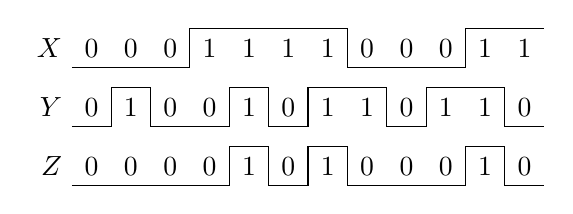
\begin{tikzpicture}
\pgfmathsetmacro{\kts}{0.5}
\pgfmathsetmacro{\kys}{0.5}
\pgfmathsetmacro{\kysep}{0.75}
\draw(0,0)node[above left]{$X$}--++(\kts,0)--++(\kts,0)--++(\kts,0)--++(0,\kys)--++(4*\kts,0)--++(0,-\kys)--++(3*\kts,0)--++(0,\kys)--++(2*\kts,0);
\draw(-\kts/2,0)
\foreach \n in {0,0,0,1,1,1,1,0,0,0,1,1}{++(\kts,0)node[above]{\n}};
\draw(0,-\kysep)node[above left]{$Y$}--++(\kts,0)--++(0,\kys)--++(\kts,0)--++(0,-\kys)--++(2*\kts,0)--++(0,\kys)--++(1*\kts,0)--++(0,-\kys)--++(1*\kts,0)--++(0,\kys)--++(2*\kts,0)--++(0,-\kys)--++(1*\kts,0)--++(0,\kys)--++(2*\kts,0)--++(0,-\kys)--++(1*\kts,0);
\draw(-\kts/2,-\kysep)
\foreach \n in {0,1,0,0,1,0,1,1,0,1,1,0}{++(\kts,0)node[above]{\n}};
\draw(0,-2*\kysep)node[above left]{$Z$}--++(4*\kts,0)--++(0,\kys)--++(\kts,0)--++(0,-\kys)--++(1*\kts,0)--++(0,\kys)--++(1*\kts,0)--++(0,-\kys)--++(3*\kts,0)--++(0,\kys)--++(1*\kts,0)--++(0,-\kys)--++(1*\kts,0);
\draw(-\kts/2,-2*\kysep)
\foreach \n in {0,0,0,0,1,0,1,0,0,0,1,0}{++(\kts,0)node[above]{\n}};
\end{tikzpicture}
\caption{ضرب گیٹ کی کارکردگی۔}
\label{شکل_بوولین_ضرب_جدول_دو_دخول}
\end{minipage}
\end{figure}

شکل  \حوالہ{شکل_بوولین_ضرب_جدول_دو_دخول}  میں دو مداخل   ضرب گیٹ کی کارکردگی  ترسیم  کی گئی ہے، جہاں \عددی{0} کو پست اور \عددی{1} کو بلند لکیر سے ظاہر کیا گیا ہے۔آپ دیکھ سکتے ہیں کہ مخارج صرف اور صرف اُس صورت بلند  ہوتا ہے جب ضرب گیٹ کے تمام مداخل بلند ہوں۔ ہم \عددی{0} کو پست اور \عددی{1} کو بلند بھی پکارتے ہیں۔ اس شکل میں  مداخل کو کسی خاص ترتیب سے  تبدیل نہیں  کیا گیا۔


ضرب گیٹ کو شکل \حوالہ{شکل_بوولین_گیٹ_بطور_سوئچ} میں بطور  عددی گیٹ یا عددی سوئچ  دکھایا گیا ہے جہاں  ایک داخلی پینا  کو قابو پینا  کا نام دیا گیا ہے جبکہ دوسرے کو   (اب بھی)  مداخل کہا گیا ہے۔ضرب گیٹ کے جدول سے واضح ہے کہ جب تک قابو پینا  \عددی{0} ہو،   خارجی پینا   \عددی{0}  رہتا ہے۔اس صورت میں   مداخل  پر موجود مواد، خارجی پینا تک نہیں پہنچ سکتا،  یعنی   اس   پر \عددی{0} یا \عددی{1}  کا مخارج پر کوئی اثر نہیں ہوتا؛  ہم کہتے  ہیں قابو پینا نے ضرب گیٹ کو معذور   کر دیا ۔اس کے برعکس اگر قابو پینا  \عددی{1} ہو تب خارجی پینا پر وہی کچھ ہوگا جو مداخل پر ہو گا؛ ہم کہتے  ہیں  ضرب گیٹ مجاز   کر دیا گیا ہے۔قابو پینا پر ایک یا صفر  سے داخلی اشارہ  (مواد) کو خارجی پینا تک پہنچنا،  ممکن یا ناممکن بنایا جا سکتا ہے۔یوں یہ ایک دروازے کی طرح کام کرتا ہے، جس   کی بنا   پر  یہ  گیٹ  کہلاتا ہے۔قابو پینا کو،  معذور اور مجاز بنانے والا پینا بھی کہتے ہیں۔شکل  \حوالہ{شکل_بوولین_گیٹ_کارکردگی}  میں ضرب   گیٹ کی  کارکردگی دکھائی گئی ہے۔آپ دیکھ سکتے ہیں کہ  صرف مجاز صورت میں مواد مخارج تک پہنچ پاتا ہے؛ معذور صورت میں مخارج ہمیشہ پست رہے گا۔

\begin{figure}
\centering
\begin{tikzpicture}
\draw(0,-2)node[above right]{مداخل}--++(2,0)--++(0.5,0.5)coordinate[pos=0.5](kk){}++(0,-0.5)--++(1.5,0)node[above left]{مخارج};
\draw[dashed](kk)--++(0,-1)--++(-1,0)node[left]{قابو};
\end{tikzpicture}\hfill
\begin{tikzpicture}
\draw(0,0)node[and port](and1){};
\draw(and1.in 1)node[left]{مداخل};
\draw(and1.in 2)--++(0,-0.5)node[below]{قابو};
\draw(and1.out)node[right]{مخارج};
\end{tikzpicture}
\caption{ضرب گیٹ بطور  سوئچ یا ایک بِٹ گیٹ۔}
\label{شکل_بوولین_گیٹ_بطور_سوئچ}
\end{figure}
%
\begin{figure}
\centering
\begin{tikzpicture}
\pgfmathsetmacro{\kts}{0.5}
\pgfmathsetmacro{\kys}{0.5}
\pgfmathsetmacro{\kysep}{0.75}
\draw(0,0)node[above left]{قابو}--++(3*\kts,0)--++(0,\kys)--++(4*\kts,0)--++(0,-\kys)--++(5*\kts,0);
\draw(-\kts/2,0)
\foreach \n in {0,0,0,1,1,1,1,0,0,0,0,0}{++(\kts,0)node[above]{\n}};
\draw(0,-\kysep)node[above left]{مداخل}--++(\kts,0)--++(0,\kys)--++(\kts,0)--++(0,-\kys)--++(2*\kts,0)--++(0,\kys)--++(1*\kts,0)--++(0,-\kys)--++(1*\kts,0)--++(0,\kys)--++(2*\kts,0)--++(0,-\kys)--++(1*\kts,0)--++(0,\kys)--++(2*\kts,0)--++(0,-\kys)--++(1*\kts,0);
\draw(-\kts/2,-\kysep)
\foreach \n in {0,1,0,0,1,0,1,1,0,1,1,0}{++(\kts,0)node[above]{\n}};
\draw(0,-2*\kysep)node[above left]{مخارج}--++(4*\kts,0)--++(0,\kys)--++(\kts,0)--++(0,-\kys)--++(1*\kts,0)--++(0,\kys)--++(1*\kts,0)--++(0,-\kys)--++(5*\kts,0);
\draw(-\kts/2,-2*\kysep)
\foreach \n in {0,0,0,0,1,0,1,0,0,0,0,0}{++(\kts,0)node[above]{\n}};
\draw(1.5*\kts,0.75)node[]{معذور};
\draw(5*\kts,0.75)node[]{مجاز};
\draw(9.5*\kts,0.75)node[]{معذور};
\end{tikzpicture}
\caption{ضرب گیٹ کی کارکردگی۔}
\label{شکل_بوولین_گیٹ_کارکردگی}
\end{figure}


\جزوحصہ{جمع گیٹ}
منطقی جمع  (بوولین جمع)  تفاعل کو جمع گیٹ  سے حاصل کیا جاتا ہے۔ دو مداخل جمع گیٹ  شکل  \حوالہ{شکل_بوولین_ضرب_دو_متغیر_گیٹ}  میں دکھایا گیا ہے۔ 
\begin{figure}
\centering
\begin{minipage}[b]{0.40\textwidth}
\centering
\begin{tikzpicture}
\draw(0,0)node[or port](or1){};
\draw(or1.in 1)node[left]{$X$}node[xshift=-0.25cm, yshift=0.75cm]{مداخل};
\draw(or1.in 2)node[left]{$Y$};
\draw(or1.out)node[right]{$Z$}node[xshift=0.25cm,yshift=1cm]{مخارج};
\end{tikzpicture}
\caption{دو مداخل جمع   گیٹ۔}
\label{شکل_بوولین_ضرب_دو_متغیر_گیٹ}
\end{minipage}\hfill
\begin{minipage}[b]{0.55\textwidth}
\centering
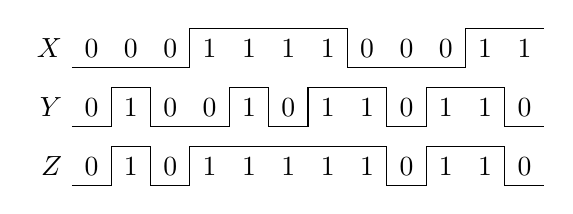
\begin{tikzpicture}
\pgfmathsetmacro{\kts}{0.5}
\pgfmathsetmacro{\kys}{0.5}
\pgfmathsetmacro{\kysep}{0.75}
\draw(0,0)node[above left]{$X$}--++(\kts,0)--++(\kts,0)--++(\kts,0)--++(0,\kys)--++(4*\kts,0)--++(0,-\kys)--++(3*\kts,0)--++(0,\kys)--++(2*\kts,0);
\draw(-\kts/2,0)
\foreach \n in {0,0,0,1,1,1,1,0,0,0,1,1}{++(\kts,0)node[above]{\n}};
\draw(0,-\kysep)node[above left]{$Y$}--++(\kts,0)--++(0,\kys)--++(\kts,0)--++(0,-\kys)--++(2*\kts,0)--++(0,\kys)--++(1*\kts,0)--++(0,-\kys)--++(1*\kts,0)--++(0,\kys)--++(2*\kts,0)--++(0,-\kys)--++(1*\kts,0)--++(0,\kys)--++(2*\kts,0)--++(0,-\kys)--++(1*\kts,0);
\draw(-\kts/2,-\kysep)
\foreach \n in {0,1,0,0,1,0,1,1,0,1,1,0}{++(\kts,0)node[above]{\n}};
\draw(0,-2*\kysep)node[above left]{$Z$}--++(1*\kts,0)--++(0,\kys)--++(\kts,0)--++(0,-\kys)--++(1*\kts,0)--++(0,\kys)--++(5*\kts,0)--++(0,-\kys)--++(1*\kts,0)--++(0,\kys)--++(2*\kts,0)--++(0,-\kys)--++(1*\kts,0);
\draw(-\kts/2,-2*\kysep)
\foreach \n in {0,1,0,1,1,1,1,1,0,1,1,0}{++(\kts,0)node[above]{\n}};
\end{tikzpicture}
\caption{جمع گیٹ کی کارکردگی۔}
\label{شکل_بوولین_جمع_جدول_دو_دخول}
\end{minipage}
\end{figure}

جمع گیٹ کی کارکردگی شکل  \حوالہ{شکل_بوولین_جمع_جدول_دو_دخول}  میں ترسیم کی  گئی ہے۔آپ دیکھ سکتے ہیں، جمع گیٹ کا مخارج اُس صورت  بلند ہوگا  جب کوئی   مداخل  بلند ہو۔

جمع گیٹ میں اگر ایک پینا کو قابو  پنیا  سمجھا جائے تو پست  قابو گیٹ کو مجاز   بنا کر ،   داخلی مواد کو مخارج تک پہنچنے کی اجازت دیتا ہے،  جبکہ بلند قابو کی صورت میں مخارج لازماً بلند رہتا ہے۔

\جزوحصہ{نفی گیٹ}
نفی  تفاعل کو نفی گیٹ سے حاصل کیا جاتا ہے،  جس کی علامت شکل \حوالہ{شکل_بوولین_نفی_گیٹ}  میں دکھائی گئی ہے، اور جو  مواد کو مخارج تک پہنچنے سے    روک نہ  پانے کے  باوجود   (نفی)  گیٹ کہلاتا ہے۔ اس کی کارکردگی شکل  \حوالہ{شکل_بوولین_نفی_کارکردگی}  میں ترسیم کی  گئی ہے۔آپ دیکھ سکتے ہیں،  نفی گیٹ کا مخارج اس کے مداخل کا اُلٹ  ہو گا۔
\begin{figure}
\centering
\begin{minipage}[b]{0.4\textwidth}
\centering
\begin{tikzpicture}
\draw(0,0)node[not port](not1){};
\draw(not1.in)node[left]{مداخل};
\draw(not1.out)node[right]{مخارج};
\end{tikzpicture}
\caption{نفی گیٹ}
\label{شکل_بوولین_نفی_گیٹ}
\end{minipage}\hfill
\begin{minipage}[b]{0.6\textwidth}
\centering
\begin{tikzpicture}
\pgfmathsetmacro{\kts}{0.5}
\pgfmathsetmacro{\kys}{0.5}
\pgfmathsetmacro{\kysep}{0.5}
\draw(0,0)node[above left]{مداخل}--++(2*\kts,0)--++(0,\kys)--++(1*\kts,0)--++(0,-\kys)--++(1*\kts,0)--++(0,\kys)--++(3*\kts,0)--++(0,-\kys)--++(2*\kys,0)--++(0,\kys)--++(\kts,0)--++(0,-\kys)--++(\kts,0)--++(0,\kys)--++(\kts,0);
\draw(-\kts/2,0)
\foreach \n in {0,0,1,0,1,1,1,0,0,1,0,1}{++(\kts,0)node[above]{\n}};
\draw(0,-\kysep)node[below left]{مخارج}--++(2*\kts,0)--++(0,-\kys)--++(1*\kts,0)--++(0,\kys)--++(1*\kts,0)--++(0,-\kys)--++(3*\kts,0)--++(0,\kys)--++(2*\kys,0)--++(0,-\kys)--++(\kts,0)--++(0,\kys)--++(\kts,0)--++(0,-\kys)--++(\kts,0);
\draw(-\kts/2,-\kysep-\kys)
\foreach \n in {1,1,0,1,0,0,0,1,1,0,1,0}{++(\kts,0)node[above]{\n}};
\end{tikzpicture}
\caption{نفی گیٹ کی کارکردگی۔}
\label{شکل_بوولین_نفی_کارکردگی}
\end{minipage}
\end{figure}

نفی تفاعل ایک  آزاد اور ایک  تابع متغیر رکھتا ہے، لہٰذا  نفی گیٹ کا ایک  مداخل اور ایک  مخارج ہو گا۔

\جزوحصہ{متعدد  مداخل گیٹ}
 ضرب گیٹ اور جمع گیٹ کے   متعدد  مداخل      ہو سکتے ہیں  (تاہم،  ان کا مخارج  ایک  ہو گا)۔  شکل  \حوالہ{شکل_بوولین_تین_مداخل_گیٹ}  میں تین مداخل کا  ضرب اور جمع گیٹ،  اور ان کے جدول دکھائے گئے ہیں۔ ضرب گیٹ کا مخارج اس  صورت بلند ہو گا جب  تمام مداخل بلند ہوں، جبکہ جمع گیٹ کا مخارج اس صورت بلند ہو گا جب کوئی بھی مداخل بلند ہو۔
\begin{figure}
\centering
\begin{tikzpicture}[minimum height=0.75cm] 
\node[or gate US, draw,logic gate inputs=nnn] (A) {}; 
\foreach \a in {1,...,3}
\draw (A.input \a -| -1,0) -- (A.input \a); 
\draw (A.output) -- ([xshift=0.5cm]A.output);
\draw(0,-2.5)node[]{
\begin{otherlanguage}{english}
\begin{tabular}{CCC|C}
A&B&C&Z\\
\toprule
0&0&0&0\\
0&0&1&1\\
0&1&0&1\\
0&1&1&1\\
1&0&0&1\\
1&0&1&1\\
1&1&0&1\\
1&1&1&1
\end{tabular}
\end{otherlanguage}
};    
\end{tikzpicture}\quad\quad\quad \quad 
\begin{tikzpicture}[minimum height=0.75cm] 
\node[and gate US, draw,logic gate inputs=nnn] (A) {}; 
\foreach \a in {1,...,3}
\draw (A.input \a -| -1,0) -- (A.input \a); 
\draw (A.output) -- ([xshift=0.5cm]A.output);
\draw(0,-2.5)node[]{
\begin{otherlanguage}{english}
\begin{tabular}{CCC|C}
A&B&C&Z\\
\toprule
0&0&0&0\\
0&0&1&0\\
0&1&0&0\\
0&1&1&0\\
1&0&0&0\\
1&0&1&0\\
1&1&0&0\\
1&1&1&1
\end{tabular}
\end{otherlanguage}
};   
\end{tikzpicture} 
\caption{تین مداخل ضرب گیٹ اور تین مداخل جمع گیٹ۔}
\label{شکل_بوولین_تین_مداخل_گیٹ}
\end{figure}


شکل \حوالہ{شکل_بوولین_دو_ضرب_سے_تین} میں دو  ضرب گیٹ   یوں جوڑے گئے ہیں کہ ایک کا مخارج دوسرے کے مداخل سے جڑا ہے۔ساتھ ہی اس دور کا بوولین جدول دیا گیا ہے۔ پہلے جدول استعمال کیے بغیر اس دور کو سمجھنے کی کوشش کرتے ہیں۔ مخارج \عددی{Z}  اس صورت  بلند ہو گا جب دائیں گیٹ کے   مداخل  \عددی{C} اور \عددی{D} دونوں بلند ہوں لیکن \عددی{D} بلند ہونے کے لئے ضروری ہے کہ بائیں گیٹ کے مداخل  \عددی{A} اور \عددی{B} دونوں بلند ہوں۔ یوں  \عددی{A}، \عددی{B} اور \عددی{C} بلند ہونے کی صورت میں مخارج \عددی{Z} بلند ہو گا؛ یہی تین مداخل ضرب گیٹ کی خاصیت ہے۔


آئیں اب جدول کو  سمجھتے ہیں۔ تین مداخل \عددی{ABC} کے خانوں کو تین ہندسوں کے ثنائی اعداد  \عددی{000} تا \عددی{111} سے  پُر کریں۔ اس کے بعد بائیں ضرب گیٹ کے مخارج  \عددی{D} کے خانے پُر کریں۔ یاد رہے   کہ یہ صرف \عددی{A} اور \عددی{B} پر منحصر ہے اور صرف اس صورت بلند ہو گا جب یہ دونوں بلند ہوں، جو آخری دو صفوں میں ہو گا۔ اس کے بعد دائیں ضرب گیٹ کے مخارج \عددی{Z} کے خانے پُر کریں۔ یہ صرف \عددی{C} اور \عددی{D} پر منحصر ہے، اور بلند صرف اس صورت ہو گا جب یہ دونوں بلند ہوں۔

ان نتائج کا جدول \حوالہ{شکل_بوولین_تین_مداخل_گیٹ} میں پیش تین مداخل ضرب گیٹ کے  جدول کے ساتھ کریں۔آپ دیکھ سکتے ہیں کہ شکل \حوالہ{شکل_بوولین_دو_ضرب_سے_تین} میں دونوں ضرب گیٹ مل کر  تین مداخل  ضرب گیٹ کا کردار ادا کرتے ہیں۔ یوں دو داخلی ضرب گیٹوں کی مدد سے زیادہ مداخل کا ضرب گیٹ حاصل کیا جا سکتا ہے۔

 شکل  \حوالہ{شکل_بوولین_دو_جمع_سے_تین}  میں دو  مداخل جمع  گیٹوں  سے  تین  مداخل  جمع گیٹ کا حصول دکھایا گیا ہے۔  یہاں \عددی{Z} صرف اس صورت پست ہو گا جب دائیں گیٹ  کے دونوں مداخل، \عددی{C} اور \عددی{D}،  پست ہوں لیکن \عددی{D} صرف اس صورت پست ہو سکتا ہے جب بائیں گیٹ کے  مداخل، \عددی{A} اور \عددی{B}، پست ہوں۔ یوں \عددی{Z} صرف اس صورت پست ہو گا جب \عددی{A}، \عددی{B}، اور \عددی{C} پست ہوں، جو تین  مداخل جمع گیٹ کی  خاصیت ہے۔

\begin{figure}
\centering
\begin{otherlanguage}{english}
\begin{tikzpicture}
\draw(0,0)node[and port](and1){} (2,-1)node[and port](and2){};
\draw(and1.in 1)--++(-0.5,0)node[left]{A} (and1.in 2)--++(-0.5,0)node[left]{B} (and1.out)node[above]{D}-| (and2.in 1) (and2.in 2)--++(-2.5,0)node[left]{C} (and2.out)node[right]{Z};
\end{tikzpicture}\quad \quad 
\begin{tikzpicture}
\draw(0,0)node[]{
\begin{tabular}{CCC|C|C}
A&B&C&D&Z\\
\toprule
0&0&0&0&0\\
0&0&1&0&0\\
0&1&0&0&0\\
0&1&1&0&0\\
1&0&0&0&0\\
1&0&1&0&0\\
1&1&0&1&0\\
1&1&1&1&1
\end{tabular}
};
\end{tikzpicture}
\end{otherlanguage}
\caption{دو مداخل ضرب گیٹ سے تین مداخل ضرب گیٹ کا حصول۔}
\label{شکل_بوولین_دو_ضرب_سے_تین}
\end{figure}
%
\begin{figure}
\centering
\begin{otherlanguage}{english}
\begin{tikzpicture}
\draw(0,0)node[or port](or1){} (2,-1)node[or port](or2){};
\draw(or1.in 1)--++(-0.5,0)node[left]{A} (or1.in 2)--++(-0.5,0)node[left]{B} (or1.out)node[above]{D}-| (or2.in 1) (or2.in 2)--++(-2.5,0)node[left]{C} (or2.out)node[right]{Z};
\end{tikzpicture}\quad \quad %
\begin{tikzpicture}
\draw(0,0)node[]{
\begin{tabular}{CCC|C|C}
A&B&C&D&Z\\
\toprule
0&0&0&0&0\\
0&0&1&0&1\\
0&1&0&1&1\\
0&1&1&1&1\\
1&0&0&1&1\\
1&0&1&1&1\\
1&1&0&1&1\\
1&1&1&1&1
\end{tabular}
};
\end{tikzpicture}
\end{otherlanguage}
\caption{دو مداخل جمع گیٹ سے تین مداخل جمع گیٹ کا حصول۔}
\label{شکل_بوولین_دو_جمع_سے_تین}
\end{figure}
%

\begin{figure}
\centering
\begin{subfigure}{1\textwidth}
\centering
\begin{tikzpicture}
\pgfmathsetmacro{\kxs}{3}
\pgfmathsetmacro{\kys}{1.25}
\draw(0,0)node[or port ,scale=1, number inputs=2](u1){u1} (0,-\kys)node[or port ,scale=1, number inputs=2](u2){u2} (\kxs,-\kys/2)node[or port ,scale=1, number inputs=2](u3){u3};
\draw(u1.in 1)node[left]{$A$} (u1.in 2)node[left]{$B$} (u2.in 1)node[left]{$C$} (u2.in 2)node[left]{$D$};
\draw(u1.out)node[above right]{$A+B$}-|(u3.in 1) (u2.out)node[below right]{$C+D$}-|(u3.in 2) (u3.out)node[right]{$(A+B)+(C+D)$};
\end{tikzpicture}
\caption{}
\end{subfigure}
\begin{subfigure}{1\textwidth}
\centering
\begin{tikzpicture}
\pgfmathsetmacro{\kxs}{3}
\pgfmathsetmacro{\kys}{1.25}
\draw(0,0)node[or port ,scale=1, number inputs=2](u4){u4} (0,-\kys)node[or port ,scale=1, number inputs=2](u5){u5} (\kxs,-\kys/2)node[and port ,scale=1, number inputs=2](u6){u6};
\draw(u4.in 1)node[left]{$A$} (u4.in 2)node[left]{$B$} (u5.in 1)node[left]{$C$} (u5.in 2)node[left]{$D$};
\draw(u4.out)node[above right]{$A+B$}-|(u6.in 1) (u5.out)node[below right]{$C+D$}-|(u6.in 2) (u6.out)node[right]{$(A+B)(C+D)$};
\end{tikzpicture}
\caption{}
\end{subfigure}
\caption{جمع اور ضرب گیٹ کے ادوار۔}
\label{شکل_بوولین_جمع_ضرب_ادوار}
\end{figure}
 جمع گیٹ اور ضرب گیٹ   پر مبنی، شکل  \حوالہ{شکل_بوولین_جمع_ضرب_ادوار}میں دکھائے  گئے    ادوار کو   مثال بنا کر،   عددی  ادوار   حل کرنا سیکھتے ہیں۔
 
 شکل  \حوالہ{شکل_بوولین_جمع_ضرب_ادوار}-الف سے آغاز کرتے ہیں جہاں  گیٹوں کو \عددی{u1}، \عددی{u2}، اور \عددی{u3} کے نام دیے گئے ہیں۔  جمع گیٹ \عددی{u1} اور \عددی{u2}  کے خارجی پنیے،           جمع گیٹ \عددی{u3}  کے داخلی  پنیوں    سے جڑے    ہیں۔ چونکہ \عددی{u1} کا مخارج \عددی{A+B} اور \عددی{u2} کا مخارج \عددی{C+D} دیگا، لہٰذا \عددی{u3} کا مخارج \عددی{(A+B)+(C+D)} یعنی \عددی{A+B+C+D} دیگا۔  


آئیں ا ب  شکل  \حوالہ{شکل_بوولین_جمع_ضرب_ادوار}-ب حل  ہیں۔ یہاں  \عددی{u4} اور \عددی{u5} کے مخارج بالترتیب \عددی{A+B} اور \عددی{C+D} دیں گے۔ چونکہ \عددی{u6} ضرب گیٹ ہے،   لہٰذا اس کا مخارج \عددی{(A+B)(C+D)} دیگا۔
\begin{figure}
\centering
\begin{subfigure}{1\textwidth}
\centering
\begin{tikzpicture}
\pgfmathsetmacro{\kxs}{3}
\pgfmathsetmacro{\kys}{1}
\draw(0,0)node[or port ,scale=1, number inputs=2](u1){u1} (0,-1.5*\kys)node[or port ,scale=1, number inputs=2](u2){u2} (\kxs,-\kys/2)node[and port ,scale=1, number inputs=2](u3){u3} (\kxs,-2*\kys)node[not port ,scale=1, number inputs=1, label={[xshift=-0.5em,yshift=-0.5em]u4}](u4){};
\draw(u1.in 1)node[left]{$A$} (u1.in 2)node[left]{$B$} (u2.in 1)node[left]{$C$} (u2.in 2)node[left]{$D$};
\draw(u1.out)node[above right]{$A+B$}-|(u3.in 1) (u2.out)node[below right]{$C+D$}-|coordinate(ktt)(u3.in 2) (u3.out)node[right]{$(A+B)(C+D)$};
\draw(ktt)|-(u4.in)  (u4.out)node[right]{$\overline{C+D}$};
\end{tikzpicture}
\caption{}
\end{subfigure}
\begin{subfigure}{1\textwidth}
\centering
\begin{tikzpicture}%[circuit logic US,minimum height=1cm] 
\pgfmathsetmacro{\kxs}{3}
\pgfmathsetmacro{\kys}{1.5}
\draw (0,0) node[or port ,scale=1, number inputs=3](u5){u5};
\draw (0,-\kys) node[or port ,scale=1, number inputs=2](u6){u6};
\draw (1*\kxs,-\kys/2) node[and port ,scale=1, number inputs=2](u7){u7};
\draw(u5.in 1)node[left]{$E$} (u5.in 2)node[left]{$F$} (u5.in 3)node[left]{$G$} 
(u6.in 1)node[left]{$H$} (u6.in 2)node[left]{$I$} (u7.out)node[right]{$(E+F+G)(H+I)$};
\draw(u5.out)node[above right]{$E+F+G$}-|(u7.in 1);
\draw(u6.out)node[below right]{$H+I$}-|(u7.in 2);
\end{tikzpicture}
\caption{}
\end{subfigure}
\caption{گیٹوں کا دوسرا دور۔}
\label{شکل_بوولین_جمع_ضرب_دوسرا_ادوار}
\end{figure}

شکل \حوالہ{شکل_بوولین_جمع_ضرب_دوسرا_ادوار}-الف  میں \عددی{u2} کا مخارج \عددی{u3} کے مداخل اور \عددی{u4} کے مداخل کے ساتھ  جڑا ہے۔ گیٹ \عددی{u1} اور \عددی{u2} کے مخارج بالترتیب \عددی{A+B} اور \عددی{C+D} ہیں۔ گیٹ \عددی{u3} کا مخارج \عددی{(A+B)(C+D)} اور \عددی{u4} کا مخارج \عددی{\overline{C+D}} ہو گا۔

 آپ  شکل \حوالہ{شکل_بوولین_جمع_ضرب_دوسرا_ادوار}-ب  کا حل،  شکل کو دیکھ کر   سمجھ سکتے ہیں۔ 


\جزوحصہ{ضرب متمم  گیٹ اور جمع متمم گیٹ}
شکل  \حوالہ{شکل_بوولین_ضرب_متمم}-الف  میں تین مداخل ضرب گیٹ کا مخارج \عددی{ABC} ہو گا، جو نفی گیٹ کا مداخل ہے، لہٰذا نفی گیٹ کا مخارج \عددی{Z=\overline{ABC}} ہوگا۔ ضرب گیٹ کے مخارج کا متمم اتنی اہمیت رکھتا ہے کہ اس کے لئے علیحدہ گیٹ  بنایا گیا ہے، جسے ضرب متمم گیٹ (یا ضد ضرب گیٹ)  کہتے ہیں اور جو شکل-ب میں  (تین مداخل کے لئے)   دکھایا گیا ہے۔

یوں دو مداخل ضرب متمم گیٹ کی مساوات درج ذیل ہو گی، جہاں \عددی{X} اور \عددی{Y} مداخل جبکہ \عددی{Z} مخارج ہے۔
\begin{align}
Z&=\overline{XY}=\overline{X}+\overline{Y}&\text{\RL{\small{(ضرب متمم)}}}
\end{align}
 ضرب گیٹ کے جدول کا متمم لینے سے ضرب متمم گیٹ  کا جدول حاصل ہو گا جو     جدول \حوالہ{جدول_بوولین_ضرب_متمم}  میں پیش کیا گیا ہے۔
\begin{table}
\centering
\begin{minipage}{0.45\textwidth}
\caption{تین مداخل ضرب متمم۔}
\label{جدول_بوولین_ضرب_متمم}
\centering
\begin{otherlanguage}{english}
\begin{tabular}{CCC|C}
A&B&C&Z\\
\toprule
0&0&0&1\\
0&0&1&1\\
0&1&0&1\\
0&1&1&1\\
1&0&0&1\\
1&0&1&1\\
1&1&0&1\\
1&1&1&0
\end{tabular}
\end{otherlanguage}
\end{minipage}\hfill
\begin{minipage}{0.45\textwidth}
\caption{تین مداخل جمع متمم۔}
\label{جدول_بوولین_جمع_متمم}
\centering
\begin{otherlanguage}{english}
\begin{tabular}{CCC|C}
A&B&C&Z\\
\toprule
0&0&0&1\\
0&0&1&0\\
0&1&0&0\\
0&1&1&0\\
1&0&0&0\\
1&0&1&0\\
1&1&0&0\\
1&1&1&0
\end{tabular}
\end{otherlanguage}
\end{minipage}
\end{table}
%
\begin{figure}
\centering
\begin{subfigure}{0.6\textwidth}
\centering
\begin{tikzpicture}%[circuit logic US,minimum height=1cm] 
\pgfmathsetmacro{\kxs}{1.75}
\pgfmathsetmacro{\kys}{1.5}
\draw(0,0)node[and port ,scale=1, number inputs=3](u1){} (\kxs,0) node[not port, scale=1, number inputs=1](u2){};
\draw(u1.in 1)node[left]{$A$} (u1.in 2)node[left]{$B$} (u1.in 3)node[left]{$C$}
 (u2.out)node[above right]{$Z=\overline{ABC}$};
\draw(u1.out)node[above right,xshift=-0.5em]{$ABC$}--(u2.in);
\end{tikzpicture}
\caption{}
\end{subfigure}
\begin{subfigure}{0.6\textwidth}
\centering
\begin{otherlanguage}{english}
\begin{tikzpicture}
\pgfmathsetmacro{\kxs}{3}
\pgfmathsetmacro{\kys}{1}
\draw(0,0)node[nand port ,scale=1, number inputs=3](u1){};
\draw(u1.in 1)node[left]{$A$} (u1.in 2)node[left]{$B$} (u1.in 3)node[left]{$C$}
 (u1.out)node[right]{$Z=\overline{ABC}$};
\end{tikzpicture}
\end{otherlanguage}
\caption{}
\end{subfigure}
\caption{ضرب متمم گیٹ یا ضد ضرب گیٹ۔}
\label{شکل_بوولین_ضرب_متمم}
\end{figure}
%
\begin{figure}
\centering
\begin{subfigure}{1\textwidth}
\centering
\begin{tikzpicture}%[circuit logic US,minimum height=1cm] 
\pgfmathsetmacro{\kxs}{2.5}
\pgfmathsetmacro{\kys}{1.5}
\draw(0,0)node[or port ,scale=1, number inputs=3](u1){} (\kxs,0) node[not port, scale=1, number inputs=1](u2){};
\draw(u1.in 1)node[left]{$A$} (u1.in 2)node[left]{$B$} (u1.in 3)node[left]{$C$}
 (u2.out)node[above right]{$Z=\overline{A+B+C}$};
\draw(u1.out)node[above right,xshift=-0.5em]{$A+B+C$}--(u2.in);
\end{tikzpicture}
\caption{}
\end{subfigure}
\begin{subfigure}{1\textwidth}
\centering
\begin{tikzpicture}
\pgfmathsetmacro{\kxs}{3}
\pgfmathsetmacro{\kys}{1}
\draw(0,0)node[nor port ,scale=1, number inputs=3](u1){};
\draw(u1.in 1)node[left]{$A$} (u1.in 2)node[left]{$B$} (u1.in 3)node[left]{$C$}
 (u1.out)node[right]{$Z=\overline{A+B+C}$};
\end{tikzpicture}
\caption{}
\end{subfigure}
\caption{جمع متمم گیٹ یا ضد جمع گیٹ۔}
\label{شکل_بوولین_جمع_متمم}
\end{figure}


شکل  \حوالہ{شکل_بوولین_جمع_متمم}-الف  میں تین مداخل  جمع  گیٹ کا مخارج \عددی{A+B+C} ہو گا، جو نفی گیٹ کا مداخل ہے، لہٰذا نفی گیٹ کا مخارج \عددی{Z=\overline{A+B+C}} ہوگا۔ جمع  گیٹ کے مخارج کا متمم اتنی اہمیت رکھتا ہے کہ اس کے لئے علیحدہ گیٹ  بنایا گیا ہے، جسے جمع  متمم گیٹ (یا ضد جمع گیٹ) کہتے ہیں اور جو شکل-ب میں (تین مداخل کے لئے)  دکھایا گیا ہے۔

یوں دو مداخل جمع متمم گیٹ کی مساوات درج ذیل ہو گی، جہاں \عددی{X} اور \عددی{Y} مداخل جبکہ \عددی{Z} مخارج ہے۔
\begin{align}
Z&=\overline{X+Y}=\overline{X}\cdot\overline{Y}&\text{\RL{\small{(جمع متمم)}}}
\end{align}
 جمع  گیٹ کے جدول کا متمم لینے سے جمع متمم گیٹ  کا جدول حاصل ہو گا جو      جدول \حوالہ{جدول_بوولین_جمع_متمم} میں  پیش کیا گیا ہے۔

%????KKKK

	اسی طرح شکل 3.15 میں تین داخلی نفی۔ضرب گیٹ دکھایا گیا ہے جسے نفی اور ضرب کے لفظ جوڑ کر نفی۔ضرب گیٹ 15 کا نام دیا گیا ہے۔
	بالکل ضرب اور جمع گیٹوں کی طرح یہ دو قسم کے گیٹ بھی دو، تین یا ان سے زیادہ مداخل والے ہو سکتے ہیں۔


	کسی بھی نفی۔جمع گیٹ کی مخارج صرف اُسی صورتہوتا ہے جب اس کے تمام مداخلہوں جبکہ کسی بھی نفی۔ضرب گیٹ کی مخارج اُس وقت تک  رہتا ہے جب تک اس کے تمام مداخلنہ ہوں۔

	شکل 3.16 میں باری باری  نفی۔جمع گیٹ اور نفی۔ضرب گیٹ کی مدد سے نفی گیٹ کا عمل حاصل کرنا دکھایا گیا ہے۔یوں نفی گیٹ کی جگہ نفی۔جمع گیٹ استعمال کیا جا سکتا ہے یا پھر اس کی جگہ نفی۔ضرب گیٹ استعمال کیا جا سکتا ہے۔
	اسی طرح شکل 3.17 میں نفی۔جمع گیٹ کی مدد سے جمع گیٹ اور ضرب گیٹ کا عمل حاصل کیا گیا ہے جبکہ شکل 3.18 میں نفی۔ضرب گیٹ استعمال کرتے ہوئے جمع گیٹ اور ضرب گیٹ کا عمل حاصل کیا گیا ہے۔



	اس شکل میں ضرب گیٹ بناتے وقت بائیں جانب سب سے نیچے نفی۔جمع گیٹ کے دونوں مداخل آپس میں جوڑ کر انہیںمتغیرہ سے منسلک کیا گیا ہے۔

	اس حصہ کے شروع میں دیکھا گیا کہ جمع، ضرب اور نفی گیٹوں کی مدد سے نفی۔جمع گیٹ اور نفی۔ضرب گیٹ حاصل کئے جا سکتے ہیں جبکہ اس حصہ کے آخر میں نفی۔جمع گیٹوں اور نفی۔ضرب گیٹوں کی مدد سے نفی گیٹ، جمع گیٹ اور ضرب گیٹ حاصل کرنا دکھلایا گیا۔

3.3.5 بلا شرکت جمع گیٹ اور نفی بلا شرکت جمع گیٹ
	بلا شرکت جمع تفاعل کو بلا شرکت جمع گیٹ 16 سے حاصل کیا جاتا ہے جس کی علامت شکل 3.19 (ا) میں دکھائی گئی ہے۔اسی طرح بلا شرکت نار تفاعل کو نفی بلا شرکت جمع گیٹ 17 کی مدد سے حاصل کیا جاتا ہے جس کی علامت شکل (ب) میں دکھائی گئی ہے۔بلا شرکت جمع گیٹ کی مخارج کے ساتھ نفی گیٹ منسلک کرنے سے بلا شرکت نفی۔جمع گیٹ حاصل کیا جا سکتا ہے۔بلا شرکت گیٹ کی کارکردگی ترسیم کے شکل میں شکل 3.20 میں دکھائی گئی ہے۔

	
	تین مداخل والے بلا شرکت جمع گیٹ کا مخارج حاصل کرتے وقت اس کے کسی دو مداخل کا بلا شرکت جمع حاصل کریں اور حاصل جواب کا تیسرے مداخل کے ساتھ بلا شرکت جمع حاصل کریں۔یہی ان تین مداخل کا بلا شرکت جمع ہے۔مساوات 3.19 میں تین مداخل والے بلا شرکت جمع گیٹ کا بوولین جدول دکھایا گیا ہے۔جیسے آپ اس جدول سے دیکھ سکتے ہیں، کسی بھی بلا شرکت جمع گیٹ کا مخارج اُس صورت بلند ہوتا ہے جب اس کے بلند مداخل کی تعداد طاق ہو۔

 
(3.19)



	طلبہ سے گزارش کی جاتی ہے کہ وہ یہاں رُک کر ان اعمال کو اچھی طرح سمجھ لیں۔

